%
% File acl2014.tex
%
% Contact: koller@ling.uni-potsdam.de, yusuke@nii.ac.jp
%%
%% Based on the style files for ACL-2013, which were, in turn,
%% Based on the style files for ACL-2012, which were, in turn,
%% based on the style files for ACL-2011, which were, in turn, 
%% based on the style files for ACL-2010, which were, in turn, 
%% based on the style files for ACL-IJCNLP-2009, which were, in turn,
%% based on the style files for EACL-2009 and IJCNLP-2008...

%% Based on the style files for EACL 2006 by 
%%e.agirre@ehu.es or Sergi.Balari@uab.es
%% and that of ACL 08 by Joakim Nivre and Noah Smith

\documentclass[11pt]{article}
\usepackage{acl2014}
\usepackage{times}
\usepackage{url}
\usepackage{latexsym}

%\setlength\titlebox{5cm}

% You can expand the titlebox if you need extra space
% to show all the authors. Please do not make the titlebox
% smaller than 5cm (the original size); we will check this
% in the camera-ready version and ask you to change it back.


\title{Instructions for ACL-2014 Proceedings}

\author{Mihael Simonič \\
  Kognitive Science \\ University of Tübingen 
  \\\And
  Nikolas Zeitler \\
  Computer Engineering  \\ University of Tübingen
  \\}

\date{}

\begin{document}
\maketitle
\begin{abstract}
LALALA abstract
\end{abstract}


\section{Introduction}\label{sec:Introduction}

Code switching (CS) is "the use of two
or more linguistic varieties in the same conversation or
interaction" \cite{scotton1977bilingual}. It is a linguistic phenomenon often present in bilingual societies.


%In the European Union 94.5\% of the population  learns English in school. Clearly, english is used as an bridge-language to communicate between europeans from different countries.  \\
Through new technologies and the fall away of border is it easier then ever to communicate with people from different countries. And of course we use english more and more on a daily basis. In the german language are words like sexy, laptop, fast food, wellness and many more widely spread[CITE FEHLT]. Furthermore could advertising not live without english anymore (e.G. Douglas - Your partner in beauty). The german language goes even a step further and invents its own english words (e.G Handy is german for mobile-phone).   \\
It is therefore interesting to look at code-switching between english and other languages. In this paper we will look at tweets containing english and spanish words. Our goal is it to find out the language for each word. \\

In this paper we perform language identification using machine learning techniques. Those techniques are able to indeficate the language of a single word without looking at the sentence. After the machine learning algorithm has indetificated the languages of each word, we try to improve the result using statistical facts of code-switching. We have with example observed that code-switching occurs very rarely in between two other words of the same language.\\VERGLEICH VERSCHIEDENER ANSÄTZE? LINEARE REGRESSION /  NEURONALE NETZE
\\
The data we are using are provided by \textit{First Workshop on Computational Approaches to Code Switching}\cite{workshop}. We have 11.400 Spanish-English tweets. Some of them are deleted or invalid thus we have XXX tweets and XXX different words. We know the language of each word in every tweet. \\
To evaluate our methods the workshop\cite{workshop} provided us with addional test- and trial-tweets.
SECTION X DOES LALALALA SECTION Y DOES LALALALA


%The tweets are from multiple different users. Thus the tweets are independent from each other. 

\section{Data}\label{sec:Data}
The data provided by \cite{workshop} contains english and spanish tweets. For each tweet are provided with how to split the words and which language this word is. Tweets contain a lot of special characters. Thus the data not only has labels for english \textit{lang1} and spanish \textit{lang2}. But also \textit{other} for emoticons, nicknames or gibberish. With example ":)", "@Ody12", or "Zaaaas" are labeled as other. The lable \textit{mixed} describes if a word contains both, spanish and english words, "ClutterDesordenLook" is such a word.  The next label is \textit{ne}, ne is a name entity. Those are proper names refering to people, places, organizations, locations or titles. The difficulty for those is that they could span above multiple words "West Coast" for example. \\
The data provides information of how to split the tweet into words. This is important in cases where punctuation marks or emoticons are directly at a word without whitespace in between with example "HEY!:)". \\
Lets say the data gives us the tweet: "@snapchateame No! Jason you look bueno!:). Next thing provides the given data the information to split the tweet into words to look like this: "snapchateame, No, Jason, you, look, bueno, :)". And finaly the data tells us which label every word gets "mixed, ambiguous, ne, lang1, lang1, lang1, lang2, other". \\

\section{Approaches}\label{sec:Approaches}
We want to find the language for every word inside a tweet. For this we use a two step approach. The first step is to train and use a machine learning algorithm. And the next step is to check its results and improve it using our knowledge about code-switching and statistical approximations. \\
Goal of the machine learning algorithm is it to look at a single word and decide which language it is. Thus we use uni- and bigrams to train the algorithm. The unigrams are every character used in the tweets, and the bigrams is a combination of every character with every character. After we obtained the uni- and bigrams we looked up every distinct word in the provided tweets. The next step was to write down a table which sowed for each word which uni- and bigrams it contains. Additional we provided the table with the language from which the word is. This way we have a table with one column containing each word. Then one column for each possible bigram and if each word contains this bigram. Lastly a column with the label from which language the word is from. We havent used trigrams since the paper \cite{multipleLanguages} already showed that trigrams wont improve the machinelearning algorithm. The next improvement is reached when using nGrams in the length of the words. But since the trigram table would have had required around 20Gbyte we did not perform this step either. The nGrams in length of words would have been resulting in a hardware problem.\\
This table is then useful in combination with the Python libraries Pandas and Sklearn.
The first machine-learning algorithm we tested was a Linear Regression. Using unigrams we had 64\% accuracy and with bigrams 84\%.  \\
\section{Evaluation}\label{sec:Evaluation}
In this section we are going to talk about how the different approaches perform solving different tasks. 
\subsection{Test Setup}
We want to know the accuracy of both approaches. The usual formula to compute the accuracy would be:
\[Accuracy = \frac{TruePos+TrueNeg}{TotalWords}\]
But we have no "TrueNegative" values. \\
Our problem does not resolve in "yes" and "no" answers because of the multiple labels "lang1","lang2","other","ne", and "mixed". Thus we compute the accuracy by computing the relative amount of correct labelled words.
\[Accuracy = \frac{TruePos}{TotalWords}\]
Our test-base consists in 5000 tweets. For every tweet we do know the correct labelling.
%taggedLanguages = list(test_data[len(test_data["taggedLanguages"])-5000:]["taggedLanguages"])


\subsection{Length Of Sentences}
The first evaluation looks at how good the accuracy is depending on the length of the sentence. Thus we label sentences of tweets and count the number of words which got correct labelled\\
Table \ref{tbl:numberOfTweets} shows how many tweets got checked for each sentence length. The number of tweets is not constant, since we picked the tweets which fitted to our desired sentence length out of our test-base.
\begin{table}[]
\centering
\label{tbl:numberOfTweets}
\begin{tabular}{c|c}
Sentence Length & Number of Tweets \\ \hline
3              & 145    \\
4              & 211    \\
5              & 265    \\
6              & 304    \\
7              & 363    \\
8              & 314    \\
9              & 275    \\
10             & 261    \\
11             & 210    \\
12             & 230    \\
13             & 181    \\
14             & 168    \\
15             & 212   
\end{tabular}
\caption{Tweets used to evaluate the result}
\end{table}
Figure \ref{fig:LRSentenceLength} shows Logistic Regession's results. The first intuitive result would be that the sentence length does not change the results. As our Logistic Regression performs on a character level. Thus ignores the sentence as a unit and looks only at single words. But the accuracy graph shows a difference. The accuracy improves with a growing sentence length.\\
But with the increasing accuracy and sentence length do two factors also change. The relative amount of "language" tags increases and the relative amount of "other" tags decreases. \\
Therefore it looks like that the Logistic Regression has problems in labelling "other", "ne", "mixed" and "ambiguous" words. Since when those words have the highest relative amount at the sentence length of three, are the results the worst. The best results occure when most of the tweet are actual words. This point is at an tweet length of 16words. Here we have 80\% spanish or english words and only 20\% different words. \\   
The relative amount of "other" changes rather quickly since usually is the "@UsersNickname" word (To talk to someone in twitter it is necessary to write @UsersNickname) labelled as "other". And usually occurs such a word only once per tweet. Also long tweets tend often to tell an actual story and not to show of emotions as short tweets tend to do. With example the three word tweet: "@Nickname :DD !!!!!" Has no "lang" tag but three times "other". %nur mal so meine Gedanken.
\begin{figure}[h]
\begin{center}
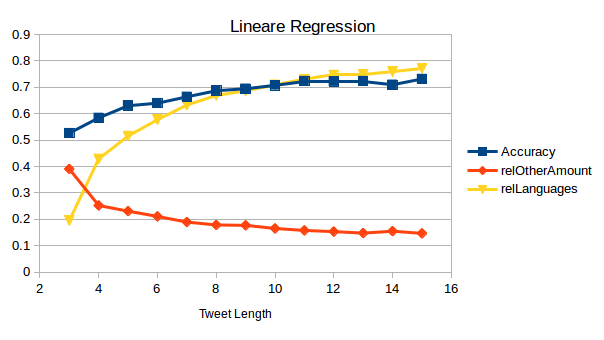
\includegraphics[scale = 0.6]{img/LinearRegressionGraf.png}
\caption{Dependency of accuracy to sentence length together with relative amount of the label "other" and relative amount of the label "lang1" or "lang2" }
\end{center} 
\label{fig:LRSentenceLength}
\end{figure}


\subsection{Accuracy labelling Gibberish}
To take a look at the strengths and weaknesses of the Logistic Regression we labelled 5000 tweets containing 69960 words. We compute the LRs accuracy per label. Our trainingsdata has six different labels. Two of them are actual langauges. Every label is shown in table \ref{tbl:accByLabel}. To compute each labels accuracy we computed the relative amount of correct labelled word for each label:
\[Accuracy_{Label} = \frac{numberOfCorrectLabels}{numberOfLabel}\] 
The results are shown in table \ref{tbl:accByLabel} \\
The table shows that the LR has problems labelling words which are no natural language (other, mixed) and name enteties (ne).  The worst performance has the LR with ambiguous word (Words which are equal in spanish and english e.g. "no") with only 9\%. But only 0.24\% of the labels are ambiguous. Thus is not much improvement for the overall system possible. 
Another good solution shows the LR for \textit{Language Detection}. This is the abbillity to recognise that the word has to be labelled with "english" or "spanish". This could be usefull to brute-force decript cypher texts with unkown keys. The LR can be used to check if the decription includes actual words or is just a failed decription containing only gibberish. The best accuaracy has the LR with english words (87\%). It seems that the bigramms perform really good with english and wors with spanish  (74\%).
\begin{table}[]
\centering
\label{tbl:accByLabel}
\begin{tabular}{ll}
Label& Accuracy \\ \hline
Other     & 0.47 \\
Ne        & 0.44 \\
Mixed     & 0.61 \\
Ambiguous & 0.09 \\
Language Detection & 0.83 \\
Spanish   & 0.74 \\
English   & 0.87 
\end{tabular}
\caption{Accuracy for different labels}
\end{table}



\section{Summary}\label{sec:Summary}

Both evaluations. Showed that the LR has problems with the label "other" but perfroms good when it comes to languages.


\begin{thebibliography}{1}
\bibitem{workshop}
Conference on Empirical Methods in Natural Language Processing ,\emph{First Workshop on Computational Approaches to Code Switching}, $emnlp2014.org/workshops/CodeSwitch/call.html$, Doha, Qatar, October 2014.


\bibitem{europa}
eurostat - Your key to European statistics, 
\emph{Foreign languages learnt per pupil in upper secondary education, 2007 and 2012}, June 2015.

\bibitem{europa}
eurostat - Your key to European statistics, 
\emph{Foreign languages learnt per pupil in upper secondary education, 2007 and 2012}, June 2015.

\bibitem{multipleLanguages}
Ben Kind, Steven Abney
\emph{Labeling the Languages of Words in Mixed-Language Documents using Weakly Supervised Methods}, University of Michigan, 2013.


\end{thebibliography}

\end{document}
